\chapter{Aufbau}

\section{Erste Planung}
Bei den anfänglichen Überlegungen stand schnell fest, dass wir uns auf zukunftsorientierte und bewährte Technologien 
stützen wollen. Nach wenigen Stunden hatten wir dann schon eine Idee wie das
UML-Diagramm auszusehen hat. Nach diesem UML-Diagramm wurde dann die erste Datenbankstruktur erstellt.

\section{Komponenten}
Unser Projekt besteht aus insgesamt drei Komponenten die miteinander kommunizieren.

\begin{itemize}
    \item \textbf{Server}: Der Server verwaltet die Daten des Projektes. Mithilfe von \textbf{HTTP} Anfragen können Daten modifiziert, verwaltet, gelöscht oder hinzugefügt werden.
    \item \textbf{Website}: Die Idee hinter der Webseite ist es, einen schnellen Überblick zu erschaffen. Skater sollen schnell 
    Skateparks finden können und auch ihre Meinung zu den jeweiligen Parks teilen können. Außerdem sollten 
    sie in der Lage sein einen Vorschlag von einem Park an die Seitenbetreiber zu schicken, welchen 
    diesen dann in die Datenbank hinzufügen können. Die Administration der Anwendung erfolgt ebenfalls
    über die Seite. 
    \item \textbf{Mobile} 
\end{itemize}

\begin{figure}[H]
    \begin{center}
      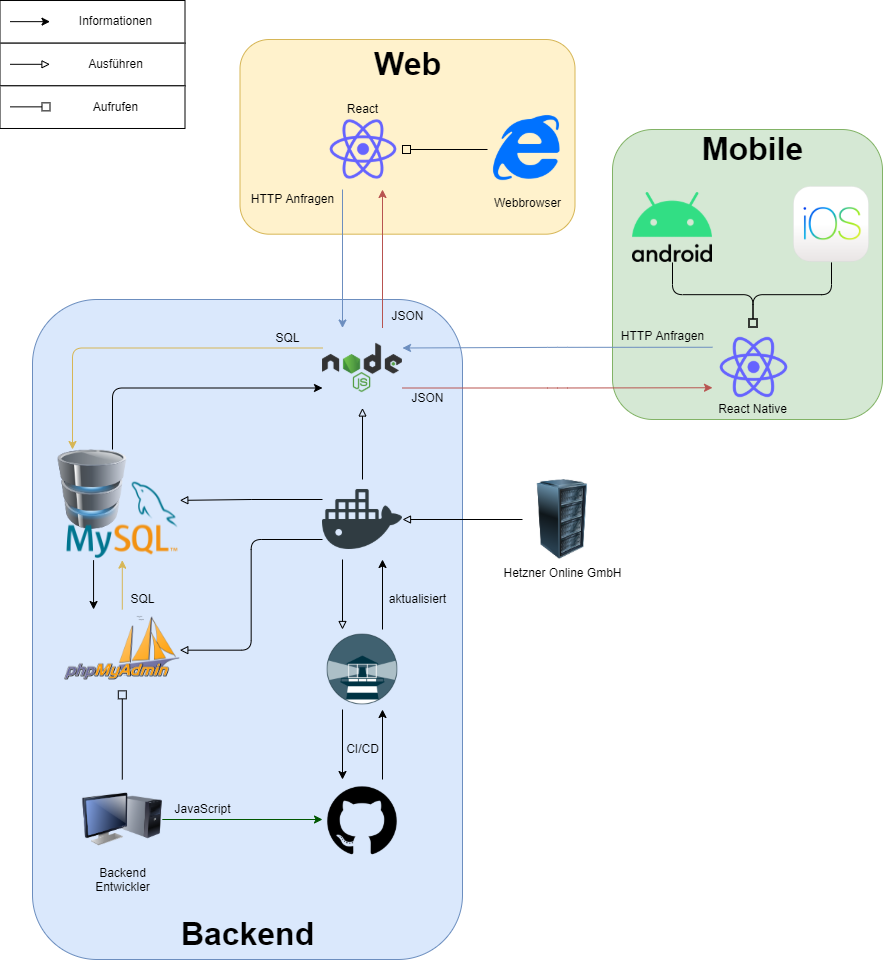
\includegraphics[width=1.0\textwidth]{Intro/Aufbau.png}
      \caption{Aufbau und Kommunikationswege des Projekts}
    \end{center}
  \end{figure}